\documentclass[a4paper,12pt]{article}
\usepackage{float}
\usepackage{amsmath, amssymb}
\usepackage{graphicx}
\usepackage{multirow}
\usepackage{booktabs}
\usepackage{geometry}
\usepackage{enumitem}
\usepackage{listings}
\usepackage{xcolor}
\geometry{margin=1in}

\begin{document}

\begin{center}
    \Large \textbf{Assignment 1} \\[6pt]
    2025.10.27
\end{center}

\section*{A. Calculations}
\subsection*{1. Compute the gravity vector}
The gravity vector $\mathbf{G}$ for estimating the torque at each joint is:
\[
\mathbf{G}(q_1, q_2, q_3) =
\begin{bmatrix}
g(m_1 r_1 c_1 + m_2(L_1 c_1 + r_2 s_{12}) + m_3(L_1 c_1 + L_2 s_{12} + r_3 s_{123})) \\
g(m_2 r_2 s_{12} + m_3(L_2 s_{12} + r_3 s_{123})) \\
g m_3 r_3 s_{123}
\end{bmatrix}
\]
where:
\[
\begin{aligned}
c_1 &= \cos(q_1) \\
s_{12} &= \sin(q_1 + q_2) \\
s_{123} &= \sin(q_1 + q_2 + q_3)
\end{aligned}
\]

\section*{B. Implementations}
\subsection*{1.[12 Points] njmoveControl() }

\begin{lstlisting}[language=C++]
void njmoveControl(GlobalVariables& gv)
{
  gv.tau = gv.kp * (gv.qd - gv.q);  // P-controller
}
\end{lstlisting}

\subsection*{2.[10 Points] Tune the controllers }

\noindent\textbf{Questions:}

\begin{enumerate}[label=(\alph*)]
    \item What kind of behaviors do you observe with different gains?
    \begin{itemize}
        \item Lower gains: There is less oscillation around the target joint state, but the error between the real joint state and the desired joint state is larger.
        \item Higher gains: The error between real joint state and the target joint state is lowers but there is more oscillation.
    \end{itemize}
    \item Why are well tuned gains different for each joint?
    
    Each joint is supporting a different amount of weight and can output different torques.
\end{enumerate}

\subsection*{3.[10 Points] Document Behavior }
Results are shown in Fig. \ref{fig:gains} and Fig. \ref{fig:taus}.

\begin{figure}[h]
  \centering

  \begin{minipage}[b]{0.48\textwidth}
    \centering
    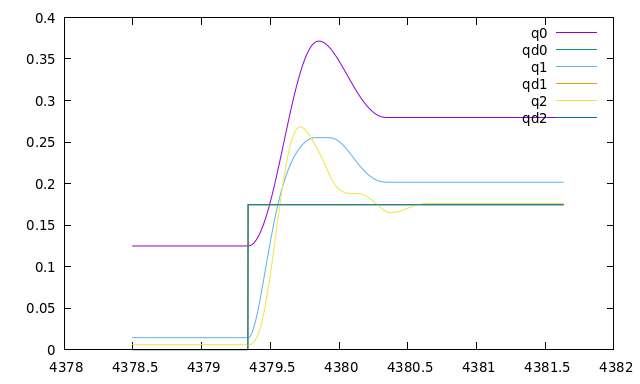
\includegraphics[width=\textwidth]{imgs/gains.png}
    \caption{Desired joint states $qd*$ and actual joint states $q*$ for \textit{njmoveControl} with Kp values: $q_1 = 400$, $q_2 = 200$, $q_3 = 25$.}
    \label{fig:gains}
  \end{minipage}
  \hfill
  \begin{minipage}[b]{0.48\textwidth}
    \centering
    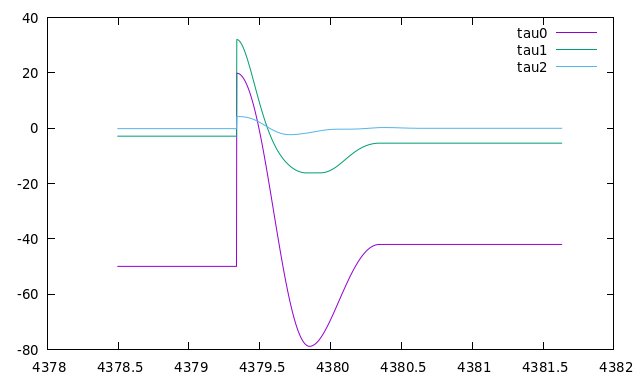
\includegraphics[width=\textwidth]{imgs/taus.png}
    \caption{Applied torques $\tau*$ for \textit{njmoveControl} with Kp values: $q_1 = 400$, $q_2 = 200$, $q_3 = 25$.}
    \label{fig:taus}
  \end{minipage}

\end{figure}

\subsection*{4.[12 Points] Calculate the gravity vector in PreprocessControl() }

\begin{lstlisting}[language=C++, breaklines=true, breakatwhitespace=true]
    float r1 = R2;
    float r2 = 0.189738;
    float r3 = R6;
    float l1 = L2;
    float l2 = L3;
    float l3 = L6;
    float m1 = M2;
    float m2 = M3 + M4 + M5;
    float m3 = M6;
    float g = -9.81;

    float c1 = cos(q1);
    float s12 = sin(q1 + q2);
    float s123 = sin(q1 + q2 + q3);

    g123[0] = g * (m1 * r1 * c1 + m2 * (l1 * c1 + r2 * s12) + m3 * (l1 * c1 + l2 * s12 + r3 * s123));
    g123[1] = g * (m2 * r2 * s12 + m3 * (l2 * s12 + r3 * s123));
    g123[2] = g * (m3 * r3 * s123);
\end{lstlisting}

\subsection*{5.[12 Points] floatControl() }

\begin{lstlisting}[language=C++, breaklines=true, breakatwhitespace=true]
    gv.tau = gv.G;
\end{lstlisting}
\subsection*{6.[12 Points] njgotoControl() }
Results are shown in \ref{fig:q_task_6} and \ref{fig:tau_task_6}

\subsection*{7.[12 Points] jgotoControl() }

The derivative component in the new PD controller reduces the oscillations caused by higher Kp gains. The gravity compensation also makes the work for the P controller easier as it does not have to account for the constant force of gravity. The results are shown in Figures \ref{fig:gains2} and \ref{fig:taus2}.

\begin{figure}[h]
  \centering

  \begin{minipage}[b]{0.48\textwidth}
    \centering
    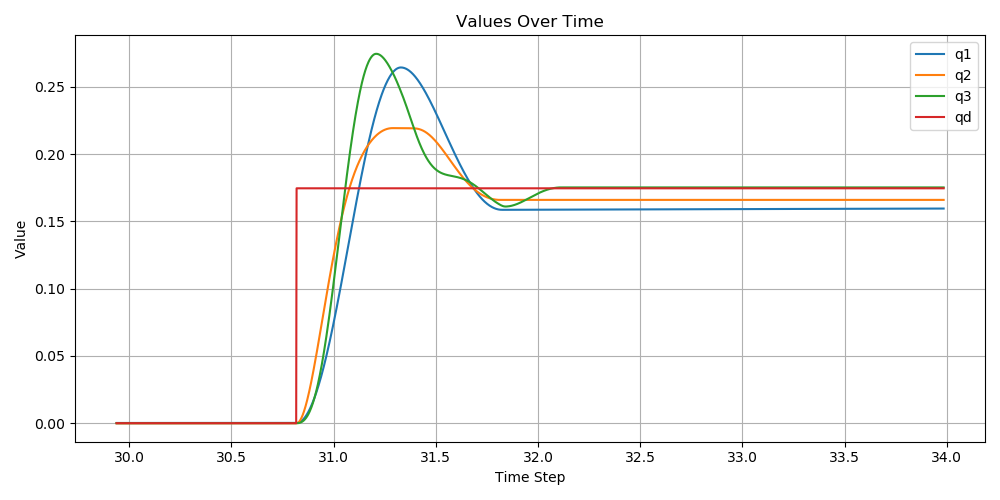
\includegraphics[width=\textwidth]{imgs/q_task_6.png}
    \caption{Desired joint states $qd*$ and actual joint states $q*$ for \textit{njgotoControl} with Kp values: $q_1 = 400$, $q_2 = 200$, $q_3 = 25$.}
    \label{fig:q_task_6}
  \end{minipage}
  \hfill
  
  \begin{minipage}[b]{0.48\textwidth}
    \centering
    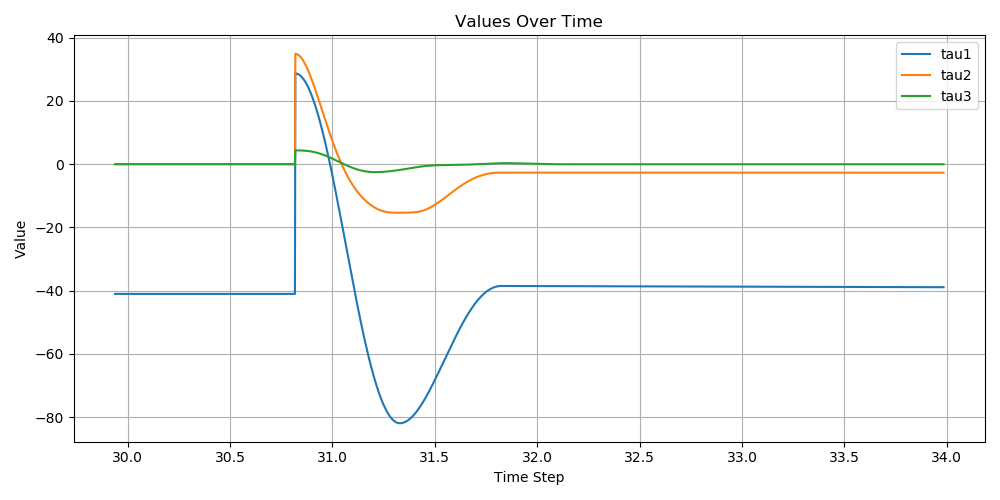
\includegraphics[width=\textwidth]{imgs/tau_task_6.png}
    \caption{Applied torques $\tau*$ for \textit{njgotoControl} with Kp values: $q_1 = 400$, $q_2 = 200$, $q_3 = 25$.}
    \label{fig:tau_task_6}
  \end{minipage}

\end{figure}

\begin{figure}[h]
  \centering

  \begin{minipage}[b]{0.48\textwidth}
    \centering
    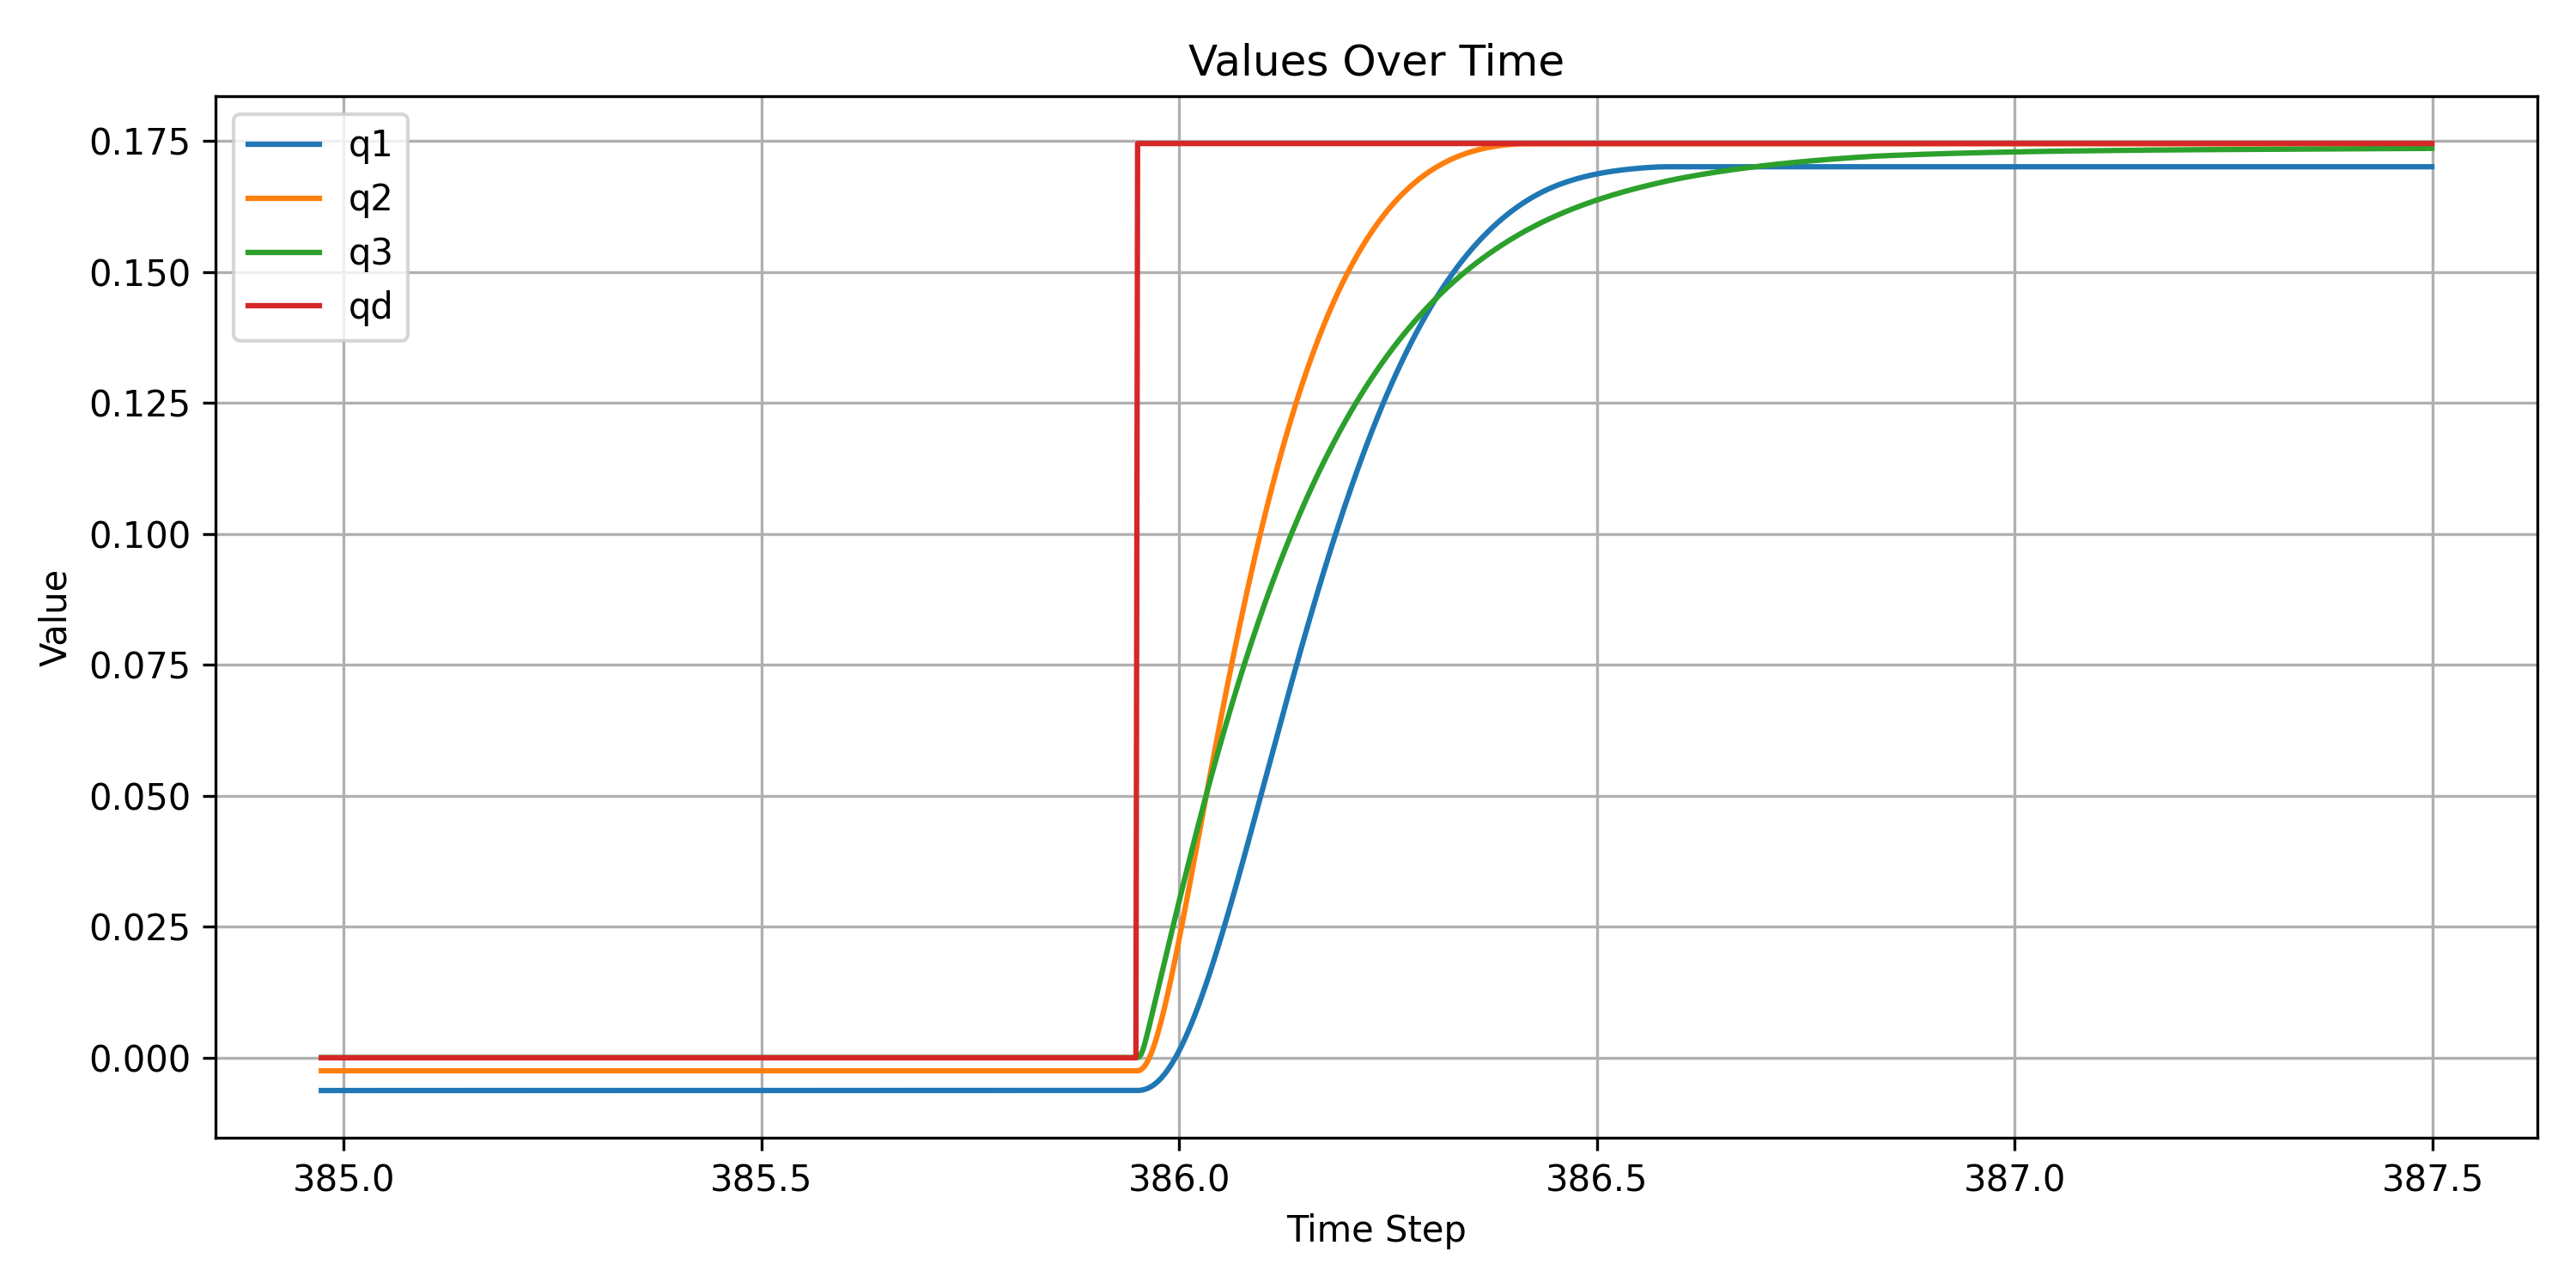
\includegraphics[width=\textwidth]{imgs/plot.png}
    \caption{Desired joint states $qd*$ and actual joint states $q*$ for \textit{jgotoControl} with Kp values: $q_1 = 600$, $q_2 = 400$, $q_3 = 200$, and Kv values: $q_1 = 100$, $q_2 = 40$, $q_3 = 40$.}
    \label{fig:gains2}
  \end{minipage}
  \hfill
  \begin{minipage}[b]{0.48\textwidth}
    \centering
    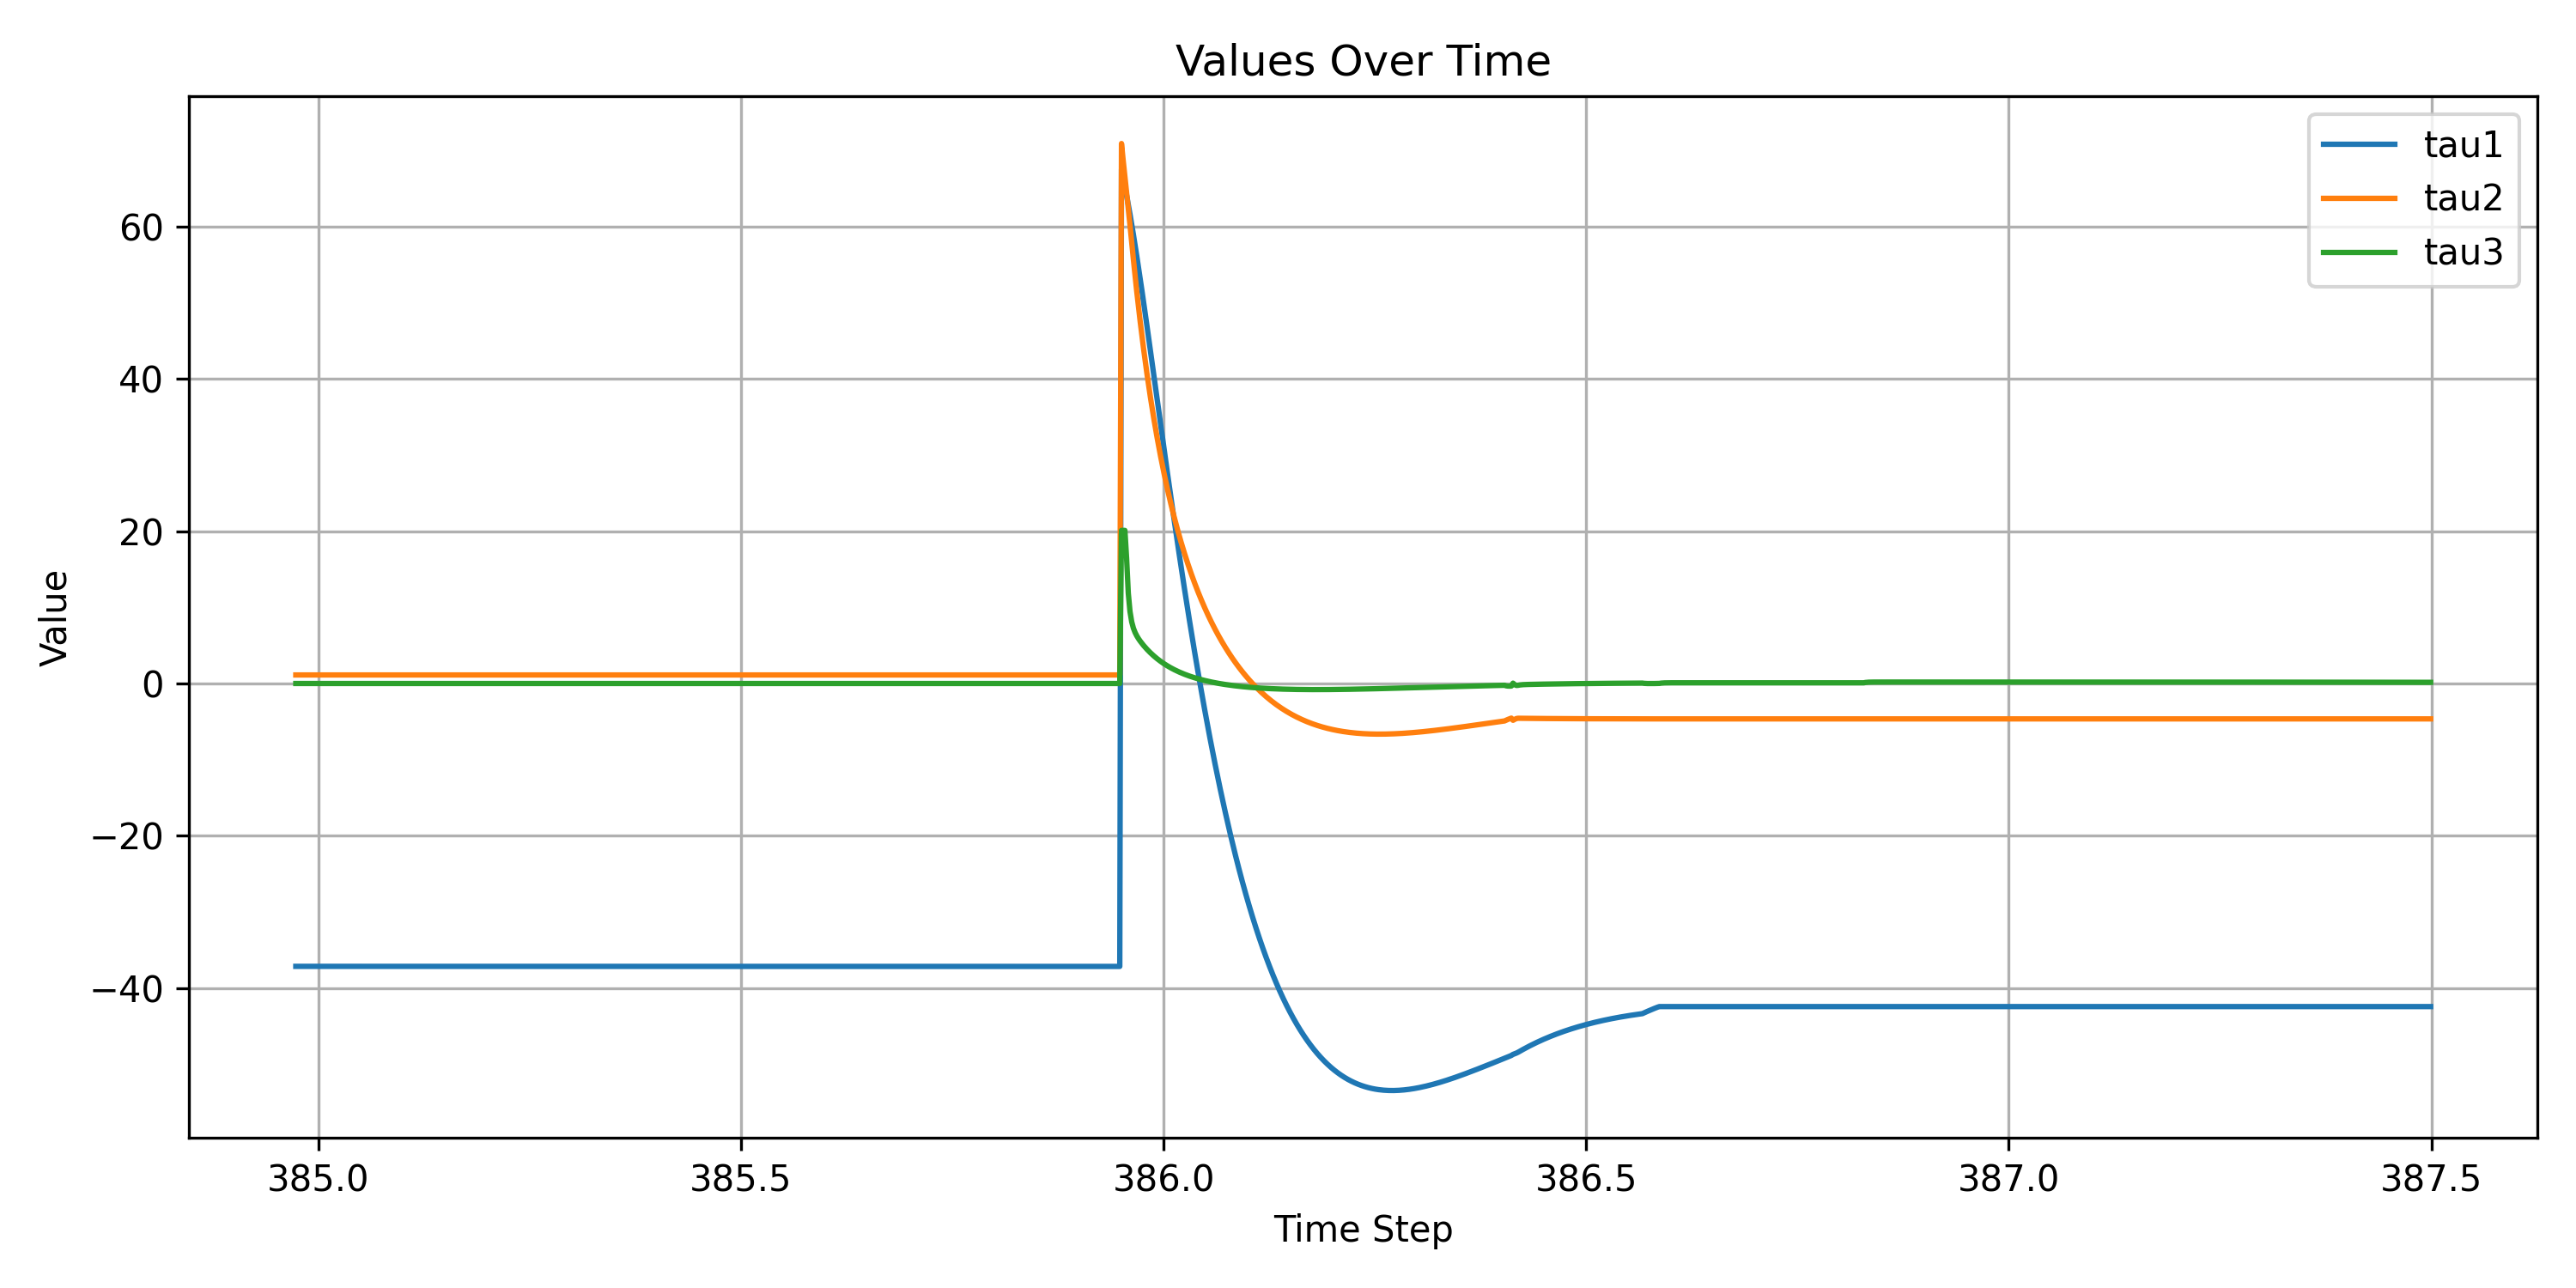
\includegraphics[width=\textwidth]{imgs/tau.png}
    \caption{Applied torques $\tau*$ for \textit{jgotoControl} with Kp values: $q_1 = 600$, $q_2 = 400$, $q_3 = 200$, and Kv values: $q_1 = 100$, $q_2 = 40$, $q_3 = 40$.}
    \label{fig:taus2}
  \end{minipage}

\end{figure}


\end{document}
